\section{Evaluation Results}
\label{sec:results}
% \todo{SV in progress}

Table~\ref{tab:results1} shows the performance of \OurApproach{} on the KGQA task in comparison with the results previously reported by  \citet{DBLP:journals/corr/abs-1803-00832}.
There is a noticeable improvement in recall (we were able to retrieve answers to 50\% of the benchmark questions), while maintaining a comparable precision score.
For the most recent QALD challenge the guidelines were updated to penalize systems that miss the correct answers, i.e., that are low in recall, which gives a clear signal of its importance for this task~\cite{DBLP:conf/semweb/UsbeckGN018}.
While it is often trivial for users to filter out a small number of incorrect answers that stem from interpretation ambiguity, it is much harder for users to recover missing correct answers.
Indeed, we showed that \OurApproach{} is able to identify correct answers that were missing even from the benchmark dataset since they were overlooked by the benchmark authors due to sampling bias.

\begin{table}
\centering
\caption{Evaluation results. (*) P of the WDAqua baseline is estimated from the reported precision of 0.59 for answered questions only. Runtime is reported in seconds per question as an average across all questions in the dataset. The distribution of runtimes for \OurApproach{} is Min: 0.01, Median: 0.67 Mean: 0.72, Max: 13.83}
\label{tab:results1}
\begin{tabular}{lcccc}
\toprule
\bf Approach & \bf P & \bf R & \bf F & \bf Runtime \\
\midrule
WDAqua & 0.22\smash{\rlap{*}} & 0.38 & 0.28    & 1.50 s/q \\
\OurApproach{} (our approach)      & 0.25 & 0.50 & 0.33    &   0.72 s/q  \\
\bottomrule
\end{tabular}
\end{table}

\subsection{Ablation study} 
Table~\ref{tab:results2} summarizes the results of our ablation study for different setups.
We report the fraction of all questions that have at least one answer that deviates from the ground truth (\emph{Total} column), questions with missing term matches (\emph{No match}) and other errors. 
Revised errors is the subset of other errors that were considered as true errors in the manual error analysis.

\begin{table*}[!t]
\caption{Ablation study results. (*) Question model results set the optimal performance for our approach assuming that the question interpretation is perfectly aligned with the ground-truth annotations. We then estimate additional (new) errors produced by each of the KGQA components separately. The experiments marked with {\bf GT} use the term URIs and question types extracted from the ground truth queries. {\bf GT span$^+$} uses spans from the ground-truth annotations and then corrects the distribution of the matched entities/properties to mimic correct question interpretation with a low-confidence tail with alternative matches. {\bf PR} (Parsed Results) stands for predictions made by question parsing and matching models (see Section \ref{sec:implementation}).}
\label{tab:results2}
%\vspace{0.2cm}
 \setlength{\tabcolsep}{5pt}
\centering\small
\begin{tabular}{ll|cccc|ccc|c|cc}
\hline
 &    \multirow{3}{*}{\bf Setup}              & \multicolumn{4}{c|}{\multirow{2}{*}{\bf Question interpretation}} &  \multirow{3}{*}{\bf P}  & \multirow{3}{*}{\bf R} & \multirow{3}{*}{\bf F}& \multicolumn{3}{c}{\bf Questions with errors}       \\
\cline{10-12}
   &    &  &  & &    &     &   &    & \multirow{2}{*}{Total}           & \multicolumn{2}{c}{New errors} \\
   \cline{3-6}\cline{11-12}
   &    & Q. type & Entity & Property & Class   &   &   &  &        & No match & Other$\rightarrow$Revised  \\
   
% \midrule
\hline
% \hline
1   & Question model*     & \multicolumn{4}{c|}{\cellcolor{lightgray}GT}            & 0.97 & 0.99 & 0.98 & \phantom{0}9\%             & --        & ~9\%   $\rightarrow$ ~5\%     \\
\hline
% \hline
2   & Question type  & PR & \multicolumn{3}{c|}{\cellcolor{lightgray} GT}    & 0.96 & 0.98 & 0.97 & 10\%             & --        & ~1\%   $\rightarrow$ ~1\%     \\
\hline
3   & Ignore classes  & \multicolumn{3}{c|}{\cellcolor{lightgray}GT}&    None      & 0.94 & 0.99 & 0.96 & 14\%             & --        & ~5\%   $\rightarrow$ ~3\%     \\
4   & Classes GT span$^+$  & \multicolumn{3}{c|}{\cellcolor{lightgray}GT}&    GT span$^+$     & 0.89 & 0.92 & 0.90 & 17\%             & \phantom{0}8\%      &  --    \\
\hline
5   & Entities GT span$^+$  & {\cellcolor{lightgray}GT}  &  GT span$^+$ & \multicolumn{2}{c|}{\cellcolor{lightgray} GT} & 0.85 & 0.88 & 0.86 & 20\%            & 10\%     & ~1\%   $\rightarrow$ ~1\%     \\
6   & Entities PR & {\cellcolor{lightgray}GT}& PR& \multicolumn{2}{c|}{\cellcolor{lightgray} GT} &  0.64 & 0.74 & 0.69 & 46\%            & 27\%     & 10\%  $\rightarrow$ ~5\%     \\
\hline
7   & Predicates GT span$^+$  & \multicolumn{2}{c}{\cellcolor{lightgray} GT} & GT span$^+$ & {\cellcolor{lightgray}GT}& 0.56 & 0.59 & 0.57 & 48\%            & 34\%     & ~5\%   $\rightarrow$ ~3\%     \\
8   & Predicates PR    & \multicolumn{2}{c}{\cellcolor{lightgray} GT} & PR & {\cellcolor{lightgray}GT} & 0.36 & 0.53 & 0.43 & 74\%            & 34\%     & 31\%  $\rightarrow$ 19\%    \\
\hline
\end{tabular}
\end{table*}

Firstly, we make sure that the relaxations in our question interpretation model hold true for the majority of questions in the benchmark dataset (95\%)
by feeding all ground truth entity, class and property URIs to the answer inference module (Setup 1 in Table~\ref{tab:results2}).
We found that only 53 test questions (5\%) require one to model the exact order of entities in the triple, i.e., subject and predicate positions.
These questions explicitly refer to a hierarchy of entity relations, such as {\tt\small dbp:doctoralStudents} and {\tt\small dbp:doctoralAdvisor} (see Figure~\ref{fig:supervision}\footnote{The numbers on top of each entity show its number of predicates and triples.}$^,$\footnote{All sample graph visualizations illustrating different error types discovered in the LC-QuAD dataset in Figure~\ref{fig:supervision}, \ref{fig:sister}, \ref{fig:rome} were generated using the LODmilla web tool, \url{http://lodmilla.sztaki.hu}~\cite{sztaki8012}, with data from the DBpedia KG.}), and their directionality has to be interpreted to correctly answer such questions.
We also recovered a set of correct answers missing from the benchmark for  relations that are symmetric by nature, but were considered only in one direction by the benchmark, e.g., {\tt\small dbo:related}, {\tt\small dbo:associatedBand}, and {\tt\small dbo:sisterStation} (see Figure~\ref{fig:sister}).

\begin{figure}[!t]
\centering
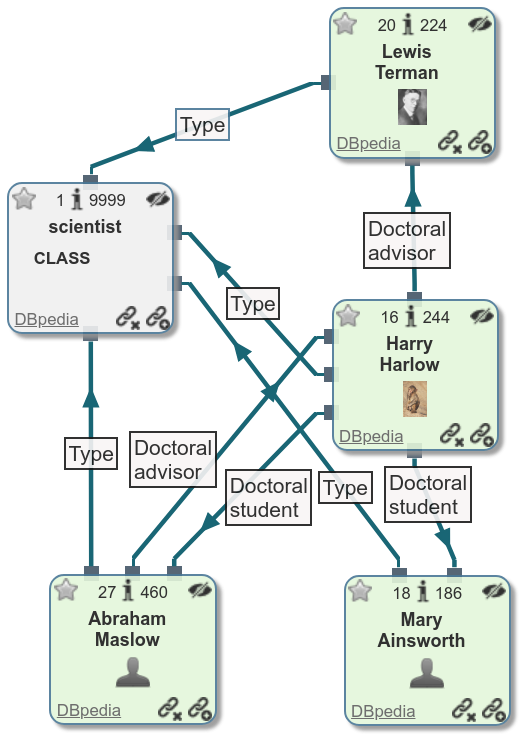
\includegraphics[width=0.37\textwidth]{figs/students.png}
\vspace{0.2cm}
\caption{\emph{Directed relation} example ({\tt\small dbp:doctoralStudents} and {\tt\small dbp:doctoralAdvisor} hierarchy) that requires modeling directionality of the relation. LC-QuAD question \#3267: ``Name the scientist whose supervisor also supervised Mary Ainsworth?'' (correct answer: Abraham Maslow) can be easily confused with a question: ``Name the scientist who supervised also the supervisor of Mary Ainsworth?'' (correct answer: Lewis Terman). LC-QuAD benchmark is not suitable for evaluating directionality interpretations, since only 35 questions (3.5\%) of the LC-QuAD test split use relations of this type, which explains high performance results of \OurApproach{} that treats all relation as undirected.}
\label{fig:supervision}
\end{figure}

\begin{figure}[!t]
\centering
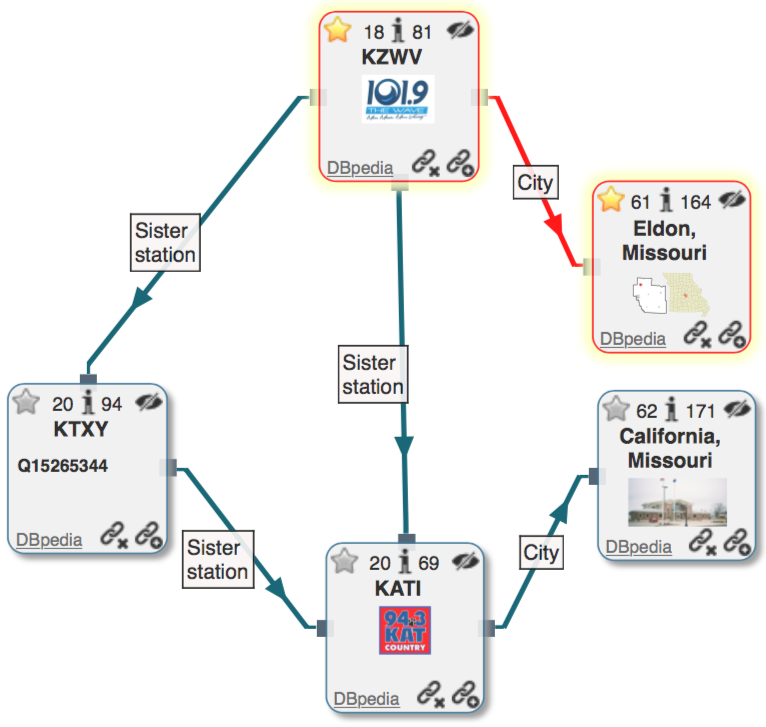
\includegraphics[width=0.48\textwidth]{figs/ktxy.png}
\caption{\emph{Undirected relation} example ({\tt\small dbo:sisterStation}) that reflects bi-directional association between the adjacent entities (Missouri radio stations). LC-QuAD question \#4486: ``In which city is the sister station of KTXY located?'' (correct answer: {\tt\small dbr:California,Missouri}, {\tt\small dbr:Missouri}; missing answer: {\tt\small dbr:Eldon,Missouri}). DBpedia does not model bi-directional relations and the relation direction is selected at random in these cases. LC-QuAD does not reflect bi-directionality either by picking only one of the directions as the correct one and rejecting correct solutions ({\tt\small dbr:KZWY} $\rightarrow$ {\tt\small dbr:Eldon,Missouri}). \OurApproach{} was able to retrieve this false negative sample due to the default undirectionality assumption built into the question interpretation model.}
\label{fig:sister}
\end{figure}

These results indicate that a more complex question model attempting to reflect structural semantics of a question in terms of the expected edges and their directions (parse graph or lambda calculus) is likely to fall short when trained on this dataset: 53 sample questions are insufficient to train a reliable supervised model that can recognize relation directions from text, which explains poor results of a slot-matching model for subgraph ranking reported on this dataset~\cite{maheshwari2018learningSHORT}.

There were only 8 errors (1\%) due to the wrong question type detected caused by misspelled or grammatically incorrect questions (row 2 in Table~\ref{tab:results2}).
Next, we experimented with removing class constraints and found that although they generally help to filter out incorrect answers (row 3) our matching function missed many correct classes even using the ground-truth spans from the benchmark annotations (row 4).

The last four evaluation setups (5--8) in Table~\ref{tab:results2} show the errors from parsing and matching reference spans to entities and predicates in the KG.
Most errors were due to missing term matches (10--34\% of questions), which indicates that the parsing and matching functions constitute the bottleneck in our end-to-end KGQA.
Even with the ground-truth span annotations for predicate references the performance is below 0.6 (34\% of questions), which indicates that relation detection is much harder than the entity linking task, which is in line with results reported by \citet{DBLP:conf/semweb/DubeyBCL18} and \citet{DBLP:journals/corr/abs-1809-10044}.

The experiments marked \textbf{GT span+} were performed by matching terms to the KG using the ground-truth span annotations, then down-scaling the confidence scores for all matches and setting the confidence score of the match used in the ground-truth query to the maximum confidence score of 1.
In this setup, all correct answers according to the benchmark were ranked at the top, which demonstrates the correctness of the message passing and score aggregation algorithm.

\subsection{Scalability analysis}

As we reported in Table~\ref{tab:results1}, \OurApproach{} is twice as fast as  the WDAqua baseline using a comparable hardware configuration. 
Figure~\ref{fig:scalability} shows the distribution of processing times and the number of examined triples per question from the LC-QuAD test split. The results are in line with the expected fast retrieval of HDT ~\cite{FMPGPA:13}, which scales linearly with the size of the graph.
Most of the questions are processed within 2 seconds (with a median and mean around 0.7s), even those  examining more than 50K triples.
Note that only 10 questions took more than 2 seconds to process and 3 of them took more than 3 seconds. These outliers end up examining a large number of alternative interpretations (up to 300K triples), which could be prevented by setting a tighter threshold. Finally, it is worth mentioning that some questions end up with no results (i.e., 0 triples accessed), but they can take up to 2 seconds for parsing and matching. 
%On the other hand, parsing and matching can take up to 2 seconds without accessing the KG.

\begin{figure}[!t]
\centering
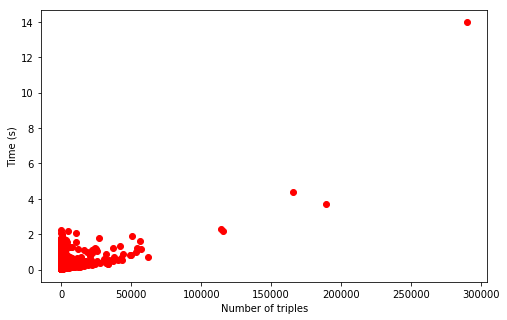
\includegraphics[width=0.48\textwidth]{figs/scalability.png}
\caption{Processing times per question from the LC-QuAD test split (Min: 0.01s Median: 0.68s Mean: 0.72s Max: 13.97s)}
\label{fig:scalability}
\end{figure}

% \todo{rephrase: Motivated by our ablation study results, we implemented the fall-backs to consider all properties, when no property could be matched to a question, and ignoring answer class information altogether rather than relying on the matching results.}

% This result was achieved by retrieving at most 500 entity URIs with the confidence threshold at least 0.7 and 50 top-ranked predicate URIs per reference, and setting the confidence threshold for the answer set entities above 0.5.

% \todo{explain HDT caching @Javier}


\subsection{Error analysis}

We sampled questions with errors (P $< 1$ or R $< 1$) for each of the setups and performed an error analysis for a total of 206 questions.
Half of the errors were due to the incompleteness of the benchmark dataset and inconsistencies in the KG (column \emph{Revised} in Table~\ref{tab:results2}).
Since the benchmark provides only a single SPARQL query per question that contains a single URI for each entity, predicate and class, all alternative though correct matches are missing, e.g., the gold-truth query using {\tt\small dbp:writer} will miss {\tt\small dbo:writer}, or match all {\tt\small dbo:languages} triples but not {\tt\small dbo:language}, etc.

% \begin{figure}[!t]
% \centering
% \includegraphics[width=0.45\textwidth]{figs/devices.png}
% \caption{\emph{Alternative class} example that demonstrates a missing answer when only a single correct class URI is considered ({\tt\small dbr:information\_appliance} and not {\tt\small dbr:device}). LC-QuAD question \#733: ``Which technological products were manufactured by Foxconn?'' (correct answers: {\tt\small dbr:Amazon\_Kindle}, {\tt\small dbr:Xbox\_One}, {\tt\small dbr:PlayStation\_4}; missing answer: {\tt\small dbr:Fire\_Phone}). \OurApproach{} was able to retrieve this false negative sample due to the semantic matching function and retaining a list of alternative URIs per class mention.}
% \label{fig:devices}
% \end{figure}

\begin{figure}[!t]
\centering
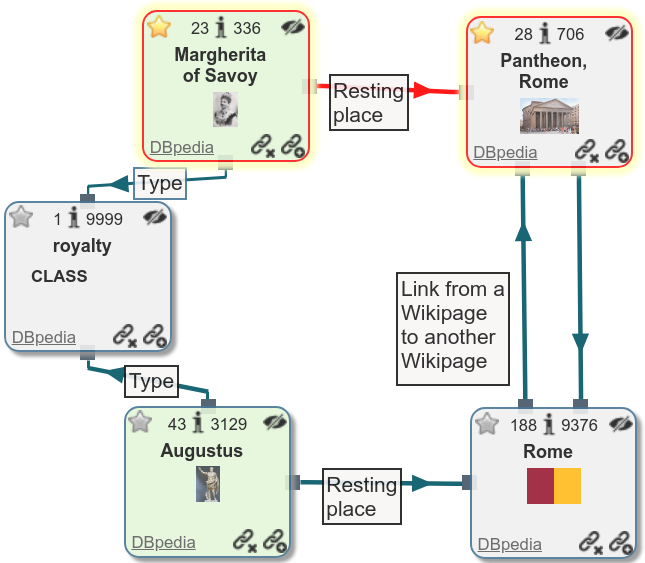
\includegraphics[width=0.48\textwidth]{figs/savoy.png}
%\vspace{0.2cm}
\caption{\emph{Alternative entity} example that demonstrates a missing answer when only a single correct entity URI is considered ({\tt\small dbr:Rome} and not {\tt\small dbr:Pantheon,Rome}).
LC-QuAD question \#261: ``Give me a count of royalties buried in Rome?'' (correct answer: {\tt\small dbr:Augustus}; missing answer: {\tt\small dbr:Margherita\_of\_Savoy}). \OurApproach{} was able to retrieve this false negative sample due to the string matching function and retaining a list of alternative URIs per entity mention.}
\label{fig:rome}
\end{figure}

\OurApproach{} was able to recover many such cases to produce additional correct answers using: (1) missing or alternative class URIs, e.g., {\tt\small dbr:Fire\_Phone} was missing from the answers for technological products manufactured by Foxconn since it was annotated as a {\tt\small device}, and not as an {\tt\small information appliance}; (2) related or alternative entity URIs, e.g., the set of royalties buried in {\tt\small dbo:Rome} should also include those buried in {\tt\small dbr:PantheonRome} (see Figure~\ref{fig:rome}); (3) alternative properties, e.g., {\tt\small dbo:hometown} as {\tt\small dbo:birthPlace}. 

% (see Figure~\ref{fig:devices})}


% \begin{figure}[!t]
% \centering
% \includegraphics[width=0.45\textwidth]{figs/race.png}
% \caption{\emph{Majority vote} example that demonstrates an effect of approximate reasoning that can retrieve alternative answers that do not fully match the input query. LC-QuAD question \#3302: ``Name the Pole driver of 1994 Spanish Grand Prix?'' (correct answer: {\tt\small dbr:Michael\_Schumacher}). \OurApproach{} also returns {\tt\small dbr:Ayrton\_Senna} as the second-best guess because he was the pole driver in many of the Grand Prix races. The model is not able to integrate other temporal facts that Senna died in an accident, while leading the 1994 San Marino Grand Prix, only a few weeks before the 1994 Spanish Grand Prix, and Michael Schumacher took over the first place in the rank afterwards.}
% \label{fig:race}
% \end{figure}

We discovered alternative answers due to the \textit{majority vote} effect, when many entities with low confidence help boost a single answer.
Majority voting can produce a best-effort guess based on the data in the KG even if the correct terms are missing from the KG or could not be recovered by the matching function, e.g., \emph{``In which time zone is Pong Pha?''} -- even if \emph{Pong Pha} is not in the KG many other locations with similar names are likely to be located in the same geographic area.
% However, this approach may also produce errors (see Figure~\ref{fig:race}).
% Such errors can be mitigated when differentiating between the activation patterns by adjusting the confidence scores with the number of evidence-source nodes, such that the candidate answers that received support from the top-match will be prefered over the candidates that received support from many nodes with a low confidence score.

Overall, our evaluation results indicate that the answer set of the LC-QuAD benchmark can be used only as a seed to estimate recall but does not provide us with a reliable metric for precision.
Attempts to further improve performance on such a dataset can lead to learning the biases embedded in the construction of the dataset, e.g., the set of relations and their directions.
\OurApproach{} is able to mitigate this pitfall by resorting to 
unsupervised message passing that collects answers from all local subgraphs containing terms matching the input question, in parallel.
